\newcommand{\geomQuery}[3] {
  \null %emptyline
  \textbf{\uppercase{#1}} 
  \begin{adjustwidth}{2.5em}{0pt}
      \begin{tabular}{p{8cm} p{2cm}}
    #3
    &
    \raisebox{-\totalheight}{\includegraphics[width=0.3\textwidth]{#2}}
  \end{tabular}
  \end{adjustwidth}
}

\chapter{Background}\label{ch:background}

\section{Monte Carlo Geometry Queries}\label{sec:mc-geom-queries}

A Monte Carlo geometry kernel must be able to robustly support the types of
geometry queries

\geomQuery{Point Containment}{plc_query.eps}{
    Given a volume and particle location, determine if the point is inside,
    outside, or on the boundary of that volume.
}

\geomQuery{Next Surface}{sc_query.eps}{
  Given a volume, particle location, and particle trajectory, determine the next
  surface of the volume that the particle intersects along with the distance to
  that intersection.
}

\geomQuery{Closest Surface}{dtb_query.eps}{
  Given a volume and particle location, determine the distance to to the nearest
  surface of the volume in any direction.
}


\geomQuery{Surface Normal}{dtb_query.eps}{
  Given a surface and particle location, determine the normal vector of the
  surface at a point closest to the particle's location.
}

\geomQuery{Measure}{dtb_query.eps}{
    Given a volume or surface in the geometry, determine properties of that entity
  such as the volume or area.
}

\geomQuery{Next Volume}{dtb_query.eps}{
  Given a volume and surface, determine the adjacent volume on the other side of
  the surface.
}

\section{Analytic Geometry Representations}\label{sec:analytic_geometry}

This section contains a discussion of common analytic geometry  representations
which are often used in native representations of Monte Carlo geometry.

\subsection{Implicit Surfaces}\label{subsec:implicit_surfaces}

An implicit surface is a multivariate function defined over an $ R^3 $ domain as:

\begin{equation}
    \Omega(R^3)\rightarrow R
\end{equation}

Implicit surfaces are rich and versatile representation of closed manifolds used
for modeling, simulation, and rendering. Additionally, implicit surfaces can be
used to generate triangle meshes for rasterization or rendering on GPUs
\cite{Sethian_1996} and can also be constructed from arbitrary triangle meshes
or point clouds \cite{Sigg_2006}. Implicit surfaces are defined using the
isocontour of a scalar function defined over all space unlike an
\textit{explicit} representation of a surface which defines the subset of space
which the boundary occupies. Intuitively it might seem wasteful for a definition
to be true for all space considering the relatively small amount of space the
object will occupy, however a number of powerful tools for geometric modeling
using these representations will be discussed in this section.

An isocontour of this function with the value, $v$, can be described as:

\begin{equation}
  \Omega(\vec{x}) - v  = 0 
\end{equation}

For simplicity, the boundary of an implicit surface is defined as the isocontour
for which $v=0$. As a result, inside of the surface will have a negative value
while any point outside of the surface will have a positive value.

Unlike their explicit counterparts, implicit representations allow complex
topologies of surfaces to be integrated into a single representation. This is in
part because the function is defined for all space.As a result they handle the
merging and separation of disparate volumes well. These properties allow for
straightforward representation of dynamics surfaces such as fluids though this
is not of concern in the area of radiation transport. In practice, implicit
surfaces are used to extract mesh representations of surfaces, re-sample the
model into some other proxy for the geometry, and render models via ray
tracing. Implicit surfaces are well-suited to these applications due to the
integrated geometric properties that can be quickly recovered from their
analytic forms.

Important geometric information needed for visualization and simulation can be
readily recovered from implicit surface representations. For example, a common
operation in particle transport is the determination of its containment by a
volume in the model. A quick evaluation of the implicit function for this point
will indicate its containment by the sign of the function.
%% Such a process is more complex in the case of an explicit or discretized
%% representation. Typically this involves casting a ray through the model and
%% counting up the intersections or relying on the orientation of triangle normals
%% to indicate an entering or exiting intersection. The oddness or eveness of the
%% number of crossings will then determine the points containment.
Additionally, the distance to nearest intersection with the surface from any
point in space can quickly be determined via the definition of a signed distance
function, $d(\vec{x})$, formally defined as:

\begin{align}
  & d(\vec{x}) = min(|\vec{x} - \vec{x_{I}}|) \\
  & \Omega(\vec(x))  \,s.t.  \,|\Omega(\vec{x})| = d(\vec(x)) 
\end{align}

\begin{align}
  d \, &- \, signed \, distance \, function \\
  \vec{x_{I}} \, &- \,nearest \, boundary \,intersection
\end{align}

\noindent
Meaning that implicit surface functions can be modified to meet the three
requirements of a signed distance function:

\begin{figure}[H]
  \begin{center}
    \begin{minipage}{.8\textwidth}
      \begin{itemize}
      \item $ \Omega(\vec{x}) = d(\vec{x}) = 0 $ for all $x$ on the surface boundary
      \item $ \Omega(\vec{x}) = -d(\vec{x}) $ for all $x$ inside the surface boundary
      \item $ \Omega(\vec{x}) = d(\vec{x}) $ for all $x$ outside the surface boundary
      \end{itemize}
    \end{minipage}
  \end{center}
\end{figure}

Implicit surfaces are often used in time-dependent simulations due to their
natural extension into a fourth dimension ($ \Omega(\vec{x},t) - v  = 0 $) and
thus their support for moving boundaries and changing topologies. Implicit
surfaces are often broken up and represented by groups of Boundary
REPresentations (BREP's). 

\subsection{Constructive Solid Geometry}\label{subsec:csg}

Native Monte Carlo geometries are commonly formed from a standard set of
well-behaved implicit surfaces known as general quadratics. These surfaces are
then combined through Boolean operations to form more complex objects (as shown
in Figure \ref{fig:csg_ex}).

\begin{figure}[h]
  \centering
  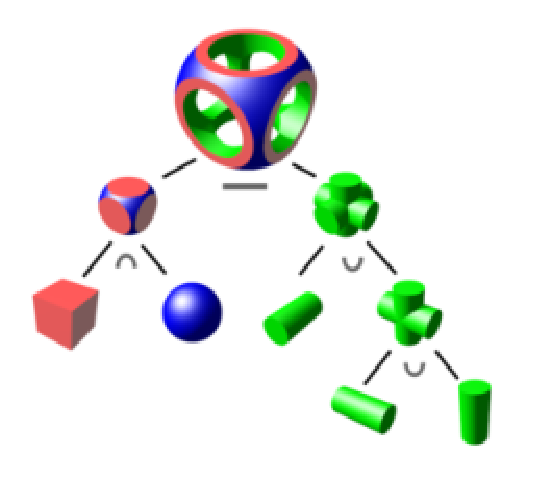
\includegraphics{csg_ex.eps}
  \caption{An example of how CSG volumes are created using Boolean combinations
    of smaller objects. The union of the three orthogonal cylinders is
    subtracted from the intersection of the box and sphere on the left to form
    the final volume at the top of the figure.}
  \label{fig:csg_ex}
\end{figure}

It is possible to construct complex geometries using CSG, but, as mentioned in
the introduction, the interface for this work is typically text-based and
defining complex volumes is a tedious and time-consuming task. Detecting
problems with the geometry definition is straightforward for the same reason
that particles can be robustly tracked through the geometry - the analytic
description of the surfaces. Fixing undefined regions of the geometry or
detecting invalid volume definitions is more difficult however.

The detection of intersections and particle containment queries in CSG
geometries is in practice computationally inexpensive for relatively simple
volume definitions, but due to the logical combinations of surfaces used to
create volumes the number of evaluations necessary to satisfy these queries is
linear with the number of surfaces in the definition. For sufficiently large and
complex models, it is not uncommon for volumes with many surfaces to be
artificially separated by planes to create two volumes with fewer surfaces in
their definition.

Visualization of CSG models can also be difficult. Because native formats for
CSG differ greatly between each Monte Carlo code, each typically comes with its
own visualization tools. These tools are typically restricted to 2D images of
the model representing a user-specified slice through the geometry. Other tools
such as MCAM \cite{Liu_2005} and McCad \cite{Tsigetamirat_2008} allow for
interactive visualization and repair of CSG models they do not provide the
accuracy of CAD modeling engines.

\subsection{CAD Geometry}

CAD systems allow for highly efficient and accurate geometric
representation. Highly complex models can be created using interactive
visualization tools represented in 3D space with a rich tool set for volume and
surface creation. These tools and the immediate visual verification of a user's
work reduces human error in model generation and design iteration.

In addition to reducing human error, CAD models provide a common domain for
analysis in other engineering domains such as fluid dynamics, heat transfer,
and structural engineering. This shared domain creates a common domain for
coupled physics simulation.

CAD also has the ability to represent free-form or higher-order surface. The use
of representations like splines and subdivision surfaces allow for more accurate
representation.

\subsection{Monte Carlo Radiation Transport on CAD Geometry}

The Direct Accelerated Geometry Monte Carlo (DAGMC) toolkit is a software
capable of Monte Carlo radiation transport directly on CAD models
\cite{Tautges_2009}. DAGMC was developed at the University of Wisconsin -
Madison. It has been coupled with many Monte Carlo codes to enable analysis on
CAD models. DAGMC relies on Cubit (and its commercial counterpart, Trelis) for CAD
modeling. Both of these CAD packages rely on the geometric modeling kernel,
ACIS.

DAGMC provides robust particle tracking for Monte Carlo transport on
arbitrarily complex CAD geometries. It accomplishes this by discretizing CAD
surfaces into sets of triangles. Volumes are then defined by any triangles which
represent bounding surfaces of a given volume. This surface mesh and the
geometric relationships between the mesh entities are stored in the Mesh
Oriented dAtaBase (MOAB) \cite{Tautges_2004}. These relationships are stored in
a hierarchical structure within MOAB, relating volumes to their surfaces,
surfaces to curves, and curves to vertices. 

It is important that geometric relationships of the mesh are maintained to
accelerate certain geometric queries on the surface mesh. For example,
\textit{Next Volume} queries are accelerated by using these relationships to
directly determine which volume a particle is passing into upon crossing a
surface rather than performing a query of the particle's location for each
volume. Other queries become more complicated due to the sheer number of
triangles needed to properly define volumes with detailed features. 

Next surface and closest to location geometry queries, for example, can be very
computationally expensive for volumes composed of hundreds of thousands or even
millions of triangles. A convenient way to think about performing geometric queries on
triangulated surfaces or volumes is to consider an equivalent CSG representation
constructed using a series of intersecting planes in place of triangles. The
structure imposed by the Boolean combinations used to define such volumes
require that each surface be checked for an intersection with the particle
trajectory. The nearest of these intersections can then be used to determine a
particle's crossing or movement to the physics event location specified by the
attached Monte Carlo code.

The problem of finding in intersection of a given particle location and
trajectory with a set of geometric primitives is known as ray tracing and is
well-studied in the field of computer graphics and animation. In this field,
data structures designed to accelerate the location of the nearest ray
intersection are applied.

\section{Ray Tracing Acceleration Data Structures}

Acceleration data structures for ray tracing are designed to rapidly narrow the
search for an intersection in virtual space given a starting position and
direction also known as a ray. This is accomplished by partitioning the space
and associating geometric primitives, most commonly triangles, with that
bounding partition. A search is performed by checking for an intersection with
the bounding partition. If the ray does not intersect with the partition, then
the set of primitives associated with that partition can be removed from the
search. If the ray does intersect with the partition, then the set of associated
primitives must be checked for intersection. Because a single separation into
two spatial partitions is often not enough to increase search efficiency, this
partitioning process is performed recursively. The result is a tree structure in
which at the top of the tree partitions are associated other partitions, known
as child nodes, rather than primitives. At the bottom of the tree exists a set of
nodes called leaves which are associated with geometric primitives. 

The search for a ray intersection then becomes a traversal of the tree
in which the children of the root node are checked for intersection. If an
intersection is found with one or both of the nodes, then the corresponding child nodes 
are checked for intersection as well. This process is repeated until leaf nodes
are reached at which point primitives are checked for intersection. Knowing that
a ray which doesn't intersect with a bounding partition cannot intersect with
any of the primitives it contains, allows many primitives to be rapidly removed
from the search and the number of intersection checks with primitives limited to
a small few. This technique reduces the algorithmic complexity of the search
from a brute force, or linear, $O(log(N_{triangles})$ to an $O(\,
log(N_{primitives}))$ search. 

\subsection{Partition Splitting Heuristics}

There are two critical components that go into the creation of spatial
partitions. The first is the selection of a candidate splitting plane which is
used to separate entities into one partition or another. The second is
the evaluation of the ``cost'' of that split should it be used. This cost is an
estimate of how good or bad the split would be. Because there is no way to know
exactly how expensive or inexpensive a split will be for the particular
simulation at hand, heuristics are used to evaluate this cost and determine the
optimal splitting plane using limited information about the local tree. This
information is typically limited to the number of primitives and bounds of the
parent partition and resulting child partitions.

The two heuristics will be addressed here - the Entity Ratio Heuristic (ERH) and the
Surface Area Heuristic (SAH). The ERH uses only the resulting number of
primitives in each child node to determine the cost of a split. The philosophy
behind this heuristic is to maintain the expected $O(log(N_{triangles})$ cost of
a ray traversal by ensuring that primitives are split as evenly as possible from
parent to child node. A form of this heuristic is presented in
Eq. \ref{eq:ERH}. This heuristic is unitless and bounded by zero and
one. This makes is possible to set both an upper and lower bound on the
unacceptable cost and a ``good enough'' cost.

\begin{figure}[H]
\begin{equation}
\label{eq:ERH}
 C = \frac{|P_{R}-P_{L}|}{(P_{R} + P_{L})} 
\end{equation}
  \begin{align*}
    C - & \,final \, cost \, evaluation \\
    P_{L} - & \, primitives\, contained\, by\, the\, left\, child  \\
    P_{R} - & \, primitives\, contained\, by\, the\, right\, child \\
  \end{align*}
  \caption{An example of the entity ratio calcution for a binary tree.}
  \label{fig:ERH}
\end{figure}

The SAH applies spatial information as well as division of primitives to the
cost evaluation. The SAH uses the surface area of candidate child partitions
relative to the current partition's surface area as an approximation for the
probability that the child will be visited after the parent volume. The explicit
form of the surface area heuristic was introduced in 1987 by Goldsmith and
Salmon \cite{Goldsmith_1987} and later formalized by MacDonald and Booth in 1990
\cite{MacDonald_1990}. Its full form is found in Equation \ref{eq:SAH}.

\begin{figure}[H]
  \begin{equation}
    C =  C_{t} + \frac{SA_{L}}{SA_{P}} |P_{L}|C_{i} +  \frac{SA_{R}}{SA_{P}} |P_{R}|C_{i}
    \label{eq:SAH}
  \end{equation}
  \begin{align*}
    C_{t} - & \,cost\, of\, traversal\, to\, child\, nodes \\
    C_{i} - & \, cost\, of\, primitive\, intersection\, check\, \\
    SA_{L} - &  \,surface\, area\, of\, left\, child \\
    P_{L} - & \, primitives\, contained\, by\, the\, left\, child  \\
    SA_{R} - & \, surface\, area\, of\, right\, child \\
    P_{R} - & \, primitives\, contained\, by\, the\, right\, child \\
    SA_{P} - & \, parent\, bounding\, volume \\
  \end{align*}
  \caption{A form of the surface area heuristic for a binary tree.}
  \label{fig:SAH}
\end{figure}

For the general case, ERH has not proved to be as effective as the SAH <REFERENCE HERE>, but it
has proven to be a useful tool in correcting the surface area heuristic for
triangle mesh features of a specific type. This scenario will be discussed further
in <INSERT HV CHAPTER HERE>.

\subsection{KD-Trees}
\label{subsec:kd-trees}
The KD-Tree or multidimensional binary search tree was originally developed as
an acceleration data structure for querying records in databases and has since
found use in other applications including speech recognition, global information
systems, and ray tracing \cite{Bentley_1975}. KD-Trees operate by using single
values to represent divisions in a dimension of the problem space. A different
dimension is split in each level of the tree, and the process is recursively
repeated until a sufficiently small number of records or entities exist within
the resulting partitions of a split, resulting in leaf nodes of the tree.

This data structure is also commonly applied to virtual 3D space for ray
intersection queries. A different dimension is split in each level of the tree
just at is done in the context of an arbitrary database. The values used for
separation of entities in the tree now represent a coordinate of a plane in that
dimension; entities are then sorted to either side of that dimension to perform
a split. First, the problem space is divided evenly in the x dimension. The two
child partitions are then divided along the y axis and the resulting children of
this division are subdivided along the z axis. Divisions are typically done in
such a way that the space of the current candidate is bisected, however it is
possible that by doing this primitive entities are divided by the plane as
well. There are a couple of ways in which this problem is handled. The first is
to simply reference any intersected primitives in both of the subdivisions. This
has the effect of creating a small overlap between the partitions and means that
some primitives may be checked for intersection more than once, but requires no
changes to the original model. The other solution is to divide the primitive
entities using the partition plane.  This solution requires alterations to the
model which may be undesirable under certain conditions and violates the
description of the KD-Tree as a pure querying structure by making modifications
to the existing model.

%% 2-D Example from Bentley1975 here %%
\begin{figure}[H]

  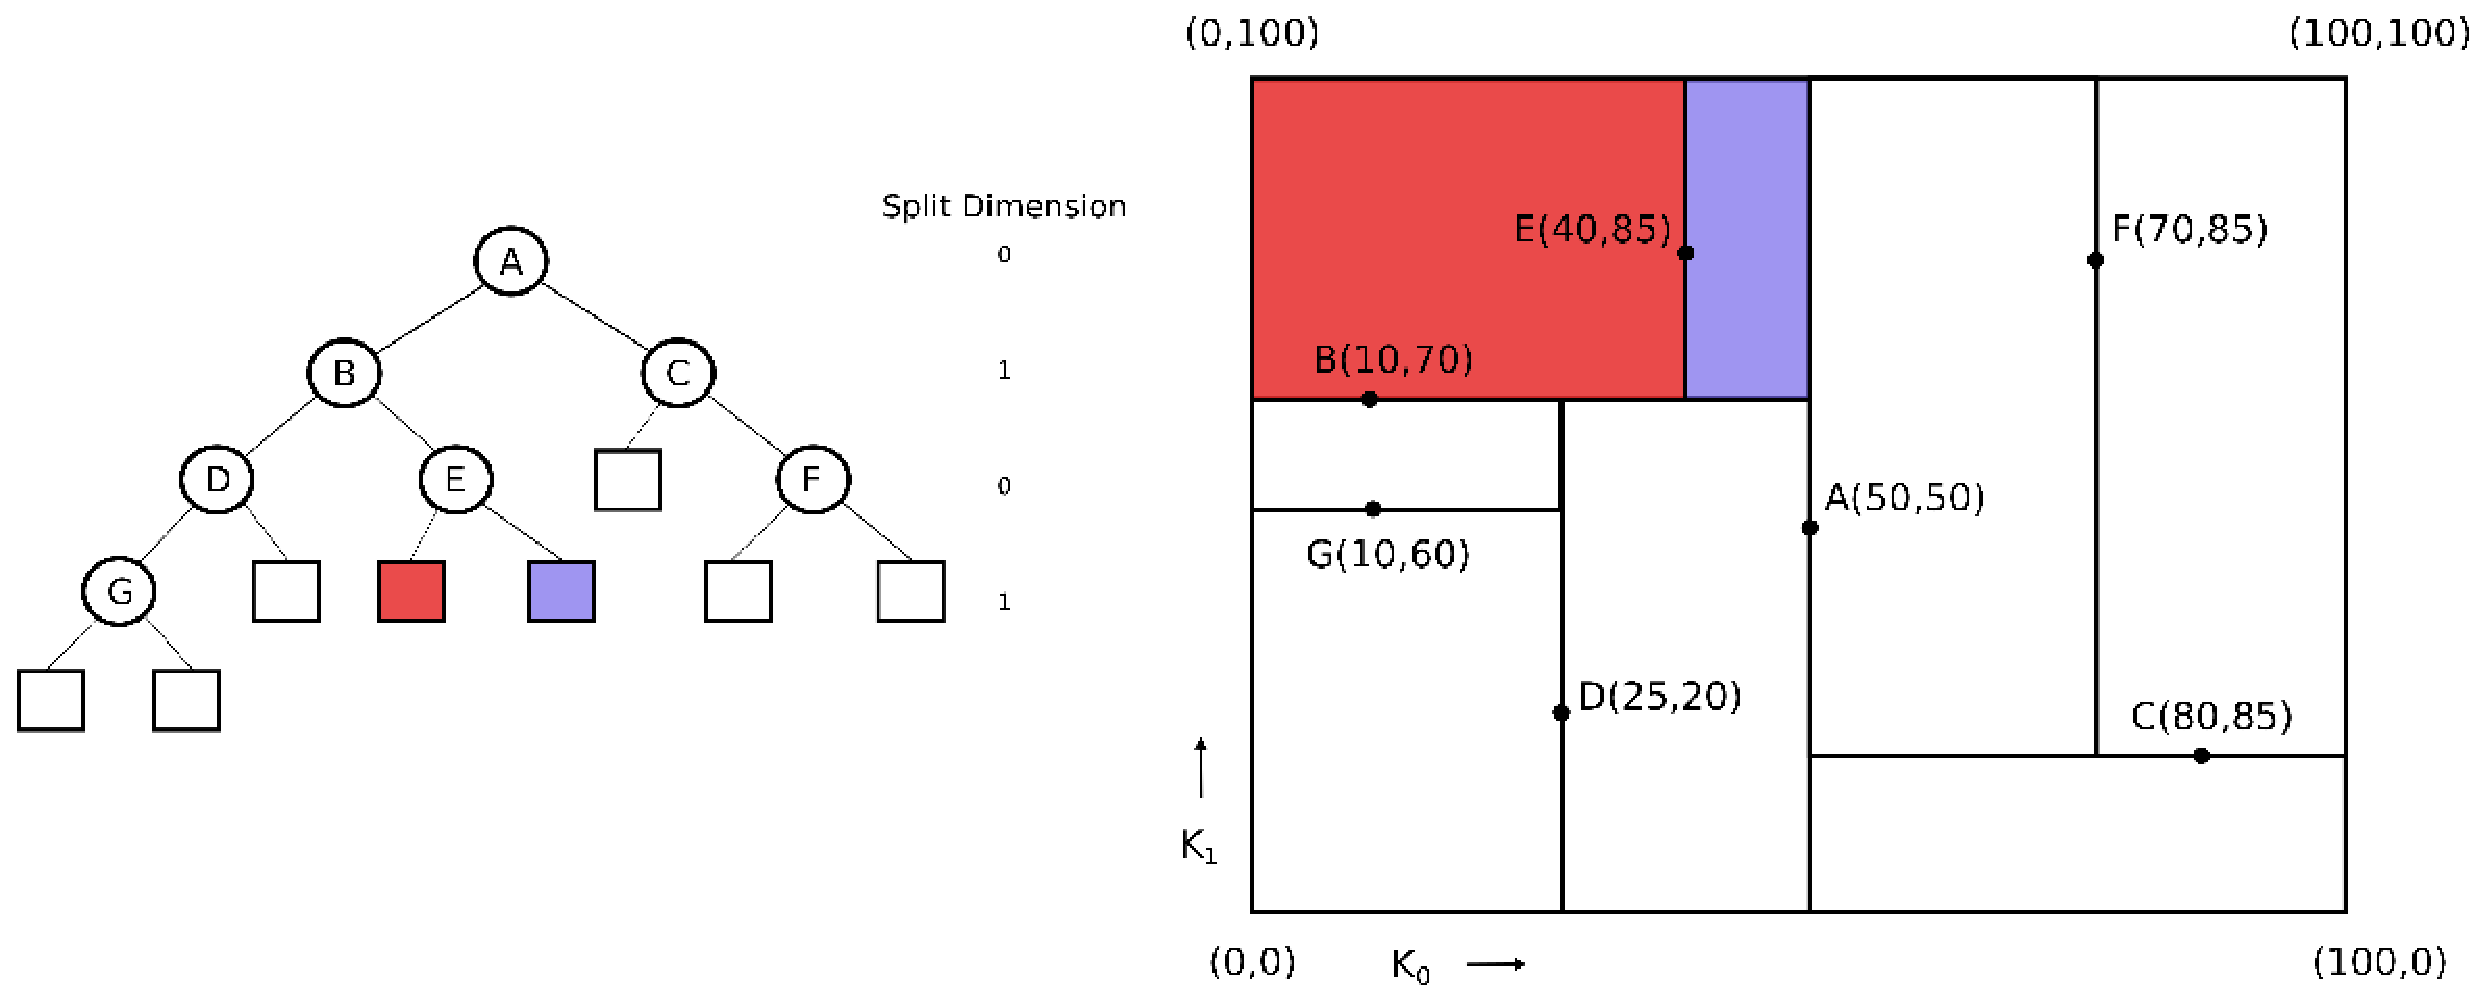
\includegraphics[scale=0.25]{2d_kd_eg.eps}
  \caption{Two dimensional KD-Tree example adapted from Bently
    et. al. \cite{Bentley_1975}. Left: Graph representation of the
    KD-Tree. HISON's are right children. LOSON's are left childre. Boxes are
    null. Right: Two dimensional space partitioned in the graph. Boxes represent
    the range of their respective sub-tree.}
  \label{fig:2D_kd_tree}
\end{figure}

KD-Trees are able to perform highly efficient due to traversal schemes developed
based on the inherent quality of KD-Trees' non-overlapping sibling nodes. As a
KD-Tree is being constructed, an ever-shrinking bounding box is being defined as
one moves deeper into the tree. At the leaves of a KD-Tree, a well-resolved
bounding box can be conceptualized using the coordinates of the last six
splitting planes visited. The conceptual construction of this box is one way to
move from node to node in a more efficient way than a more standard depth-first
approach used in tree traversal. The partitions whose planes are used to
construct this conceptual box can be linked to the current partition in order
maintain a spatially localized search within the hierarchy. These links are
referred to as neighbor links and, as shown by Samet et. al.\cite{Samet_1989},
can be used to significantly reduce traversal costs in the KD-Tree. During
traversal if a leaf is visited its neighbor links can be used to direct the
query to either the next adjacent leaf or a nearby interior node in the tree
thus avoiding a depth-first style traversal in which the next step upon visiting
a leaf node is to return to the root node of the tree and continue. These
neighbor links take advantage of the idea that if a leaf node is visited, but
the desired intersection is not found, then it is likely that the desired
intersection is close to the current leaf location. In this way, one can avoid
large amounts of unnecessary shallow and middle level tree traversal steps.

KD-Trees are frequently cited as being able to provide the best ray tracing
performance to date \cite{Ernst_2007,Hurley_2002,Havran_2000}. In particular,
KD-Trees are noted as being better equipped to handle models with highly varying
triangle sizes/densities. In practice, KD-Trees tend to be very deep and can
consume relatively high amounts of memory compared to other acceleration data
structures. 

\subsubsection{Bounding Volume Hierarchies}%%Status: Done%%
\label{subsec:BVH}
The initial concept of using the bounding volume construct as a pre-check for
ray-intersection with CSG objects was introduced by Weghorst in 1984
\cite{Weghorst_1984}. Weghorst explored the possibility of using bounding
spheres and bounding boxes to contain geometric objects. This work also went so
far as to create a hierarchy out of the object-based bounding volumes, noting the
importance of hierarchically joining bounding volumes near to each other in space
so as not to have parent volumes containing large amounts of empty space between them.

\begin{figure}[H]
  \centering
  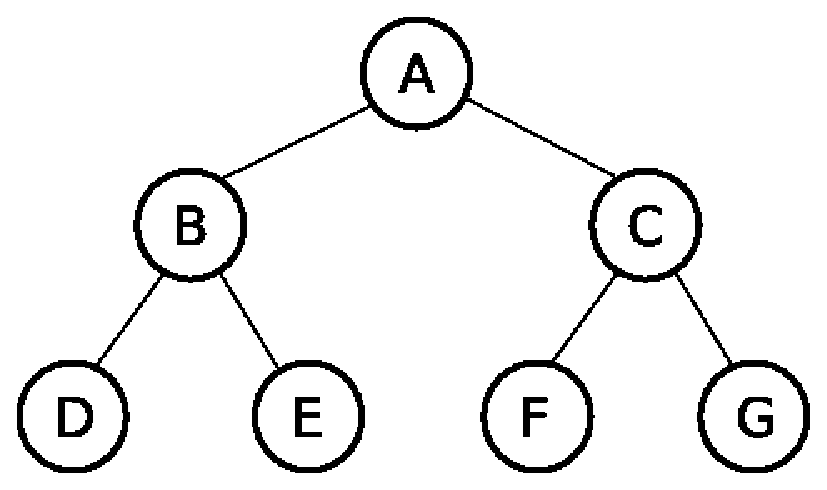
\includegraphics[scale=0.3]{binary_graph.eps}
  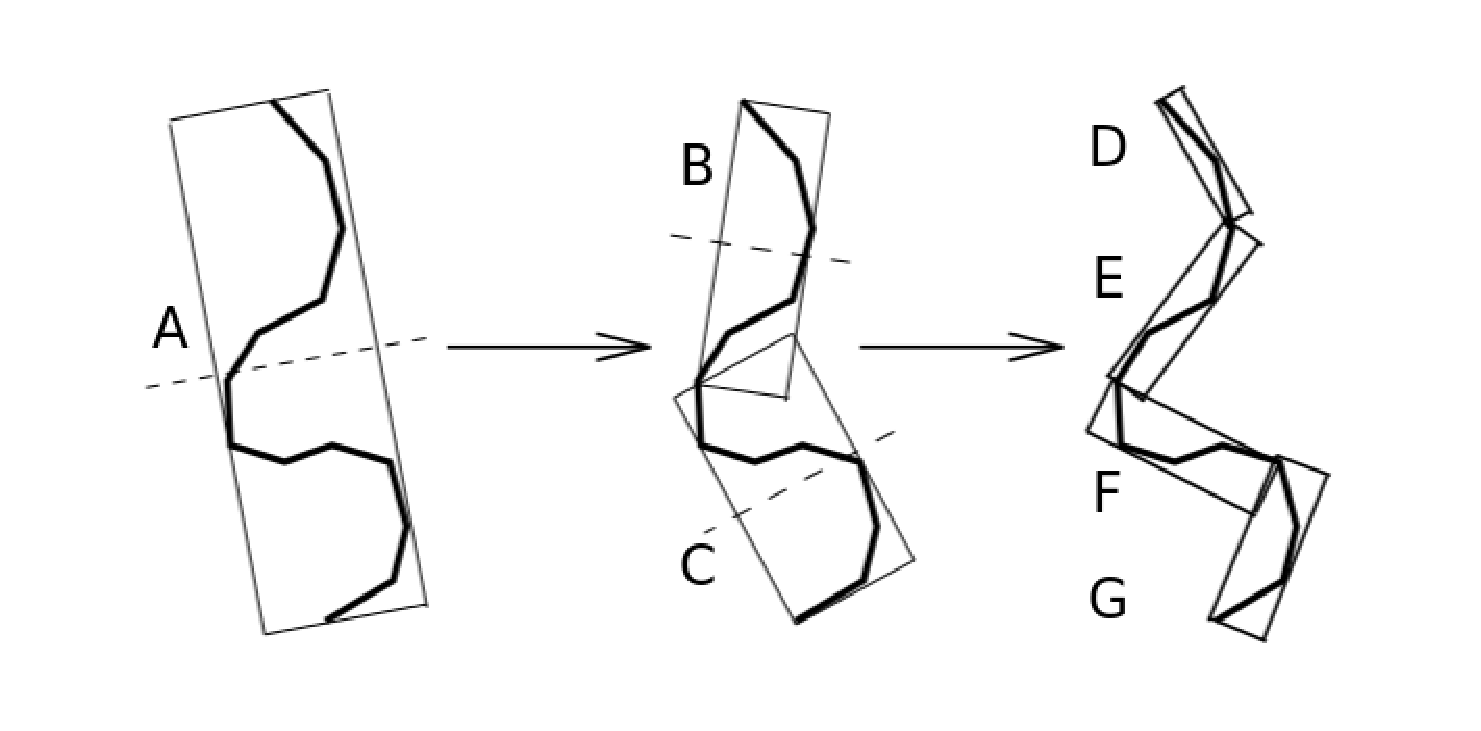
\includegraphics[scale=0.3, trim = 0 50 0 0 ]{bvh_2d_ex.eps}
  \caption{Two dimensional BVH example adapted from Gottschalk 1996 \cite{Gottschalk_1996}}
  \label{fig:2D_bvh}
\end{figure}

In Weghorst's exploration of sphere and box bounding volumes it was found that
while spherical bounding volumes are not as computationally expensive to check
for ray intersections than bounding boxes. The latter generally provide a
tighter fit to the objects they contain, and this decreases the chance of wasted
ray-volume intersection checks for rays which intersect the bounding volume but
not the object it contains. When considering the application of bounding volumes
to a discretized analytic surface represented by a triangle mesh, this becomes
even more important as BVHs become deeper when constructed on large numbers of
primitive entities and more ray-volume intersection checks are performed to
reach leaf nodes. Even applied to analytic objects, this effect was reflected
in the results of Weghorts's work strongly enough to show that bounding boxes
provided better performance in accelerating the ray intersection process than
bounding spheres.

Two forms of BVHs are commonly applied in ray tracing problems: Axis-Aligned
Bounding Boxes (AABBs) and Oriented Bounding Boxes (OBBs). AABBs are boxes whose
orientation is restricted such that their faces are parallel to the global
planes of the problem space. Given a set of points to contain, tightly fitting
axis aligned boxes are straightforward to construct and overlaps between the
children of a parent box are minimal. Their simple representation results in a
relatively low memory footprint and straightforward, robust ray-intersection
tests. Unlike AABBs, the faces of oriented bounding boxes are allowed take any
orientation relative to the global axes in order to enclose their set of
primitives as tightly as possible. Several robust methods for determining the
orientation of a box for best fit to a set of primitives have been discovered
\cite{Gottschalk_1996,ORourke_1985}. OBBs are better for avoiding superfluous
ray-box intersections that might otherwise occur for an AABB. They also
more quickly conform to the full set of enclosed primitives as the boxes are
recursively divided. By orienting their axes with the local set of primitives
they are bounding, candidate splitting planes, usually based on the current box
axes, are more effective at separating primitive entities and reaching leaf
conditions quickly. This leads to more shallow hierarchies making the worst-case
number of intersection tests lower than for an AABB hierarchy on
average. While a shallow hierarchy might indicate a smaller memory footprint,
OBBs require one to store some extra information about their orientation
relative to the global axes making this assumption difficult to consistently
prove.

One disadvantage of using OBBs is that the ray-box intersection check requires
an extra step in transformation of the ray to the oriented axes of the box in
question. The information needed for transformation of the ray basis must
be constructed and applied to the ray before the box intersection can continue
as it would for an axis aligned box. Thus, for a given ray query, an OBB hierarchy may
have fewer intersection checks to perform than an AABB hierarchy, but the
intersection checks are inherently more expensive than in the case of OBBs. In
practice, AABBs are commonly used in BVH's for their simplicity of
implementation and well-researched ray intersection algorithms. Other reasons
for this preference will be discussed later in Section \ref{subsec:arch}.

There are multiple approaches to constructing such data structures given a set
of geometric primitives, but only ``top-down'' approaches will be discussed
here. A top-down approach begins with the construction of a single bounding
volume enclosing all primitives which will be part of the tree. At this point,
child boxes of this root volume are created by selecting a splitting plane for
the box which divides the primitives contained by the current bounding volume
into two subsets. This process is then repeated until leaf conditions are
met. The selection of candidate splitting planes and the selection of a final
plane for splitting based on its estimated worth can greatly affect the
performance of the data structure. An infinite number of planes could be
tested to find the optimal plane for dividing the entities between the two child
volumes, but even if one were to encounter such a splitting plane, it can be
difficult to identify the plane as such without more knowledge about the final
tree structure. As a result, a limited set of planes is tested for the best
split based on a set of assumptions about the problem at hand and the heuristics
being used to evaluate split costs. The most common method for split plane
candidates is median plane splitting in which a bounding volume is split in half
for each axes of the current bounding volume. The splitting planes are then
evaluated and the split with the lowest cost is selected.

One difficulty that BVH's of any type face is that of overlapping sibling
bounding volumes. Overlapping sibling volumes can cause additional box
intersection checks in a similar manner to loosely fitting bounding volumes. If
a ray enters a region of overlapping sibling volumes, this causes the children
of both boxes to be checked despite the fact that the ray will eventually only
intersect with primitives contained by only one of the boxes. Overlaps are difficult to
avoid, however, due to the reality that volumes are required to contain discrete
elements for robustness, not just a section of the virtual space. Simply put, if
the splitting plane of a bounding volume goes through one of the geometric
primitives, there will be an overlap in the resulting child volumes. This
inefficiency can be exacerbated by the structure of triangulated objects the
BVHs are being formed around. Fortunately overlaps of sibling AABBs are
typically limited to the size of perhaps one or two geometric primitives and
there are other ways to cope with this problem.

The spatial BVH variant (SBVH) was introduced by Stich et. al. in 2009
\cite{Stich_2009} with an additional complexity to the node splitting step. As
candidate split planes are considered, the duplication of triangles (or
geometric primitives) to be contained in both resulting nodes. This grants much
more freedom when considering how a node should be partitioned. Conversely, this
extra freedom expands the search space of an optimal split plane for the node,
making the process more complex. The relatively simple application of this
method is performed by considering both splits in which triangle duplication is
prohibited and splits in which it is allowed. In the scenario for which triangle
duplication is prohibited, the set of candidate planes is equivalent to that of
a standard BVH building algorithm. Stich applies the surface area heuristic for
the purpose of his publication. In the case where reference duplication is
allowed, the search for a splitting plane is much more open - as previously
mentioned. In fact, the search becomes fundamentally aligned with the search for
a spatial split as might be found in a KD-Tree implementation. The optimal
splitting plane is then selected via a comparison of the SAH cost for all
candidate split planes - spatial or traditional. Secondary heuristics are used
to limit reference splitting in an effort properly manage the data structure's
memory footprint. The result of the SBVH is a hierarchy which can be traversed
just like any other BVH but with significantly reduced sibling volume
overlaps. The general effect of the allowance for reference splitting during
construction is more tightly fitting bounding volumes and reduced sibling volume
overlap. Their results consistently show significant improvement over other
methods, ranging anywhere from (20-100\%).\cite{Stich_2009}

Bounding volume hierarcies are favoered in the field of ray tracing for their
lower memory footprints and well-developed parallel building schemes. These
features are of great import for systems with limited memory, such as GPUs, and
applications with intent for realtime viewing or interaction. These requirements
do not necessarily apply to the realm of Monte Carlo particle tracking which is
commonly performed on CPUs which have more memory available relative to GPUs.

%% The BVH is currently the most commonly employed acceleration data structure for ray tracing due to its reduced memory footprint in comparison to the other data structures discussed in this chapter. They are relatively simple to implement for the performance they are able to provide and have a smaller footprint relative to most other ray tracing acceleration data structures.

\subsubsection{Octrees}%%Status:Done%%
\label{subsec:octree}

Octrees are a partitioning scheme in which cuboid bounding boxes known, also
known as voxels, are used to partition the 3D problem space into the 8 quadrants
defined by the global axes and extents of the parent voxel. These 8 voxels are
then linked as children of the parent voxel. This process is repeated
recursively until leaf conditions are met in which a sufficiently small number
of primitives is contained within the current voxel.

This spatial subdivision technique is commonly used to efficiently index
data in 3-D space.\cite{Glassner_1989} Octrees are somewhat like KD-trees in
that their divisions are spatial, their partitions contain no overlaps, and the
placement of entities in nodes occurs in a similar manner to that of KD-trees,
but each node is represented by a closed bounding volume as in a BVH.

Octrees can consume a large amount of memory relative to the other data
structures previously discussed in this chapter. It is often possible that
voxels may be completely devoid of underlying entities. There are typically many
voxels containing no primitive references but may be required to exist as part
of the data structure. This results in many voxels being stored in memory which
aren't useful other than to verify that the space they contain is
empty. Additionally, geometric primitives may be referenced multiple times if
they intersect multiple nodes thus increasing the required memory storage with
the same consequence as seen in KD-Tree traversl with the possibility of a
primitive being checked more than once upon traversal. The memory footprint is
mostly of concern in applications for visualization on GPUs - though specialized methods for Octree applications on these architectures do exist.

\begin{figure}[H]
  \centering
  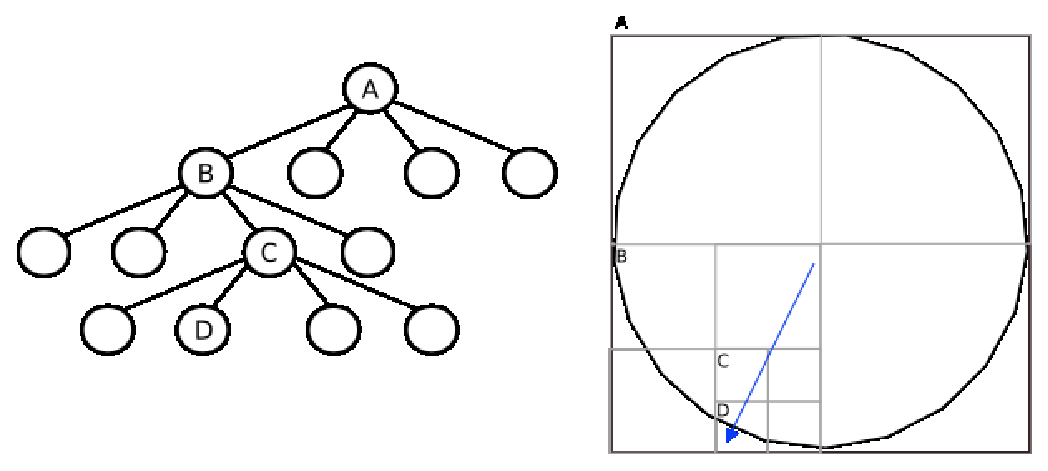
\includegraphics[scale=0.65]{octree_2d_ex.eps}
  \caption{Two dimensional Octree example of a top-down ray fire traversal for a simple geometric object.}
  \label{fig:2D_octree}
\end{figure}

One advantage of octrees is the regular nature of the partitions. The
value of a node in hierarchies such as these (or in the BVH for that matter)
lies in its ability to remove candidate space from the query, yet a voxel can
only accomplish this if rays strike the voxel. The result is that one measure of
a voxel's value can be described by the ratio of its probability of an
intersection check to the space it will exclude from the query search or its
volume. In a problem with a uniform ray distribution, the probablity of a ray to
intersect a given voxel can be related to a voxel's surface area. Thus cubic
voxels have the most favorable ratio possible based on their geometry. The
uniformity of voxel properties provide a predictable nature of the octree which
is advantageous when traversing the data structure as well.

The predictable size and location of any given node in the tree determined from
the root node properties also provides a fast lookup of the deepest node in the
tree containing a point in space. This is helpful in providing a starting point
for ray traversal which is deeper than the root node, allowing one to potentially avoid some traversal steps in the shallow levels of the tree. Additionally, octrees have non-overlapping nodes which allows
for efficient traversal schemes similar to the neighbor linked traversal done in
KD-trees. These traversals are conceptually similar to that of the KD-tree's but
typically employ some form of Morton encoding to determine which node in the
octree the ray should visit next \cite{Revelles_2000}. Other traversal
techniques allow the octree to avoid creating and traversing nodes containing
empty space which can significantly reduce its memory footprint in cases where
internal nodes of the tree aren't required to define some spatial dataset as
mentioned above \cite{Samet_1989}. These methods are often applied in GPU
environments due to the limited memory available there. Octrees are often used
to store spatial data fields as well and naturally provide a higher resolution of the field
near boundaries of volume as the voxels become smaller in that
region which can be seen in Figure \ref{fig:2D_octree}.

As mentioned above, octrees are known for having prohibitively large memory
footprints than other data structures, but they can also be used advantageously
for a combined purpose if a problem requires the storage of one or more
well-resolved data fields near volume boundaries as well as the capability for
ray tracing traversals similar in nature to those of the KD-tree.

\subsection{Architecture Based Acceleration}%%Status: Pending%%
\label{subsec:arch}

This section will focus on the advantages of vectorization implementations or
Single Instruction Multiple Data (SIMD) programming. When considering
the problem of parallelism in computing, programmers focus on one of two areas:
\textit{functional parallelism} or \textit{data parallelism}. Functional
parallelism describes the method of performing multiple operations in parallel
on many processors while data parllelism describes operation on multiple
data sets at the same time on a single processor. SIMD is a form of data
parllelism in which, as the name indicates, the same set of numerical operations
are performed on multiple sets of data in parallel. Chipsets with support for
SIMD instructions became very popular in the mid-1990s as the home PCs became
more common and demand for multimedia-related performance increased. In
response, many CPU manufacturers at the time such as Intel, IBM, and Motorola
began to release products with SIMD instruction sets. The most powerful of which
was Intel's Streaming SIMD Extensions (SSE). Over time, CPU clock speed became
the larger focus of many manufacturers due to dramatic gains in processor
speed. As processor speed increases began to wane or push the limit of current
cooling technology in the early 2000's, a new shift toward mult-core designs
occurred. Currently, as CPU clock speeds remain somewhat steady in multi-core
systems, a focus on single-thread performance via SIMD has returned to great
effect. Newer SIMD instruction sets such as Intel's Advanced Vector Extensions
(AVX or AVX2) have been able to provide double the width of operable data,
allowing for a theoretical doubling of performance in SIMD enabled codes
\cite{Hughes_2015}.

SIMD execution has found use in many different areas including medical imaging,
financial analysis, database management, computer visualization, and physical
simulation. As is the case in any problem well-suited to parallel programming,
all of these applications perform the same set of computations many times on
similarly structured sets of data. This kind of situation arises quite often in applications
related to modeling or and visualization of virtual space. One indicator of a
problem which would benefit from parallel programming is the presence of a few
common sets of operations done many times or in a recursive manner. Traversal of
ray tracing data structures is well suited for SIMD operations as it relies
heavily on the performance of a few key operations: hierarchy ray-node
intersections and ray-primitive intersections. The ability to perform intersection
checks of many nodes at once or many triangles at once has clear benefit when
satisfying geometric queries in simulations or renderings which may require
billions of these queries. Several demonstrations of ray-tracing data structures
adapted to take advantage of SIMD-enabled optimization on modern CPUs have
already been developed.

\begin{figure}
  \centering
  \includegraphics[scale=0.6]{simd_ex.eps}
  \caption{Concept of data parallelism using SIMD. Adapted from Intel's
    documentation on the advanced vector extensions instruction
    set. \cite{Intel_AVX}}
  \label{fig:simd}
\end{figure}

An early implementation of SIMD used to intersect a ray with many triangles at
the leaf nodes of a KD-Tree was performed by Hurley in 2002
\cite{Hurley_2002}. This implementation demonstrated a significant improvement in
ray-primitive intersection performance and established many significant
observations about the utilization of SIMD commands within ray tracing
applications. Despite the fact that the cost of primitive intersection checks
was reduced, most of the time spent satisfying the ray query was spent in
traversal of the hierarchy to the leaf nodes. Noting that the number of
triangles in the KD-Tree's leaf nodes were small in comparison to the SIMD
registry width, Hurley described two ways in which to further exploit data
parallelism of SIMD in ray tracing.

One method is to traverse and intersect multiple rays at the same time. This is
refereed to as the N:1 approach. The other is to intersect many nodes with a
single ray which is referred to as the 1:N approach. A key characteristic for
the former method is that the group of rays being intersected has very similar
traversal paths through the hierarchy so they may be grouped together in a
packet for a narrow traversal path. This property is known as often described as
``ray coherence''. Branching off of Hurley's work, Wald demonstrated that rays
can be effectively grouped into packets and traversed in a binary space
partitioning tree (a modified KD-Tree) to achieve performance equal to that the
high-end graphics hardware of the time \cite{Wald_2001}.

Today, as more realistic physical effects are being applied to ray tracing
kernels such as light-scattering surfaces, smoke effects, or fog, rays paths
become less coherent, meaning that the same or very similar primary rays will
not necessarily follow similar paths through the model or its underlying
acceleration hierarchies. Due to this problem-dependent lack of ray coherency,
the latter method of data parallelism in which one ray is intersected with many
hierarchy elements in a single step has been revisited revisited. Wald wisely
observed that taking advantage of SIMD operations in traversal of a KD-Tree is
difficult due to the nature of the partition. He goes on to state that the
KD-Tree's superior serial performance in comparison to that of serial BVH
implementations drove reluctance to move away from the KD-Tree and resulted in
the establishment of ray packets. \cite{Wald_2008} Both Wald and Dammertz
\cite{Dammertz_2008}, concurrently presented implementations of SIMD enabled
traversal and primitive intersection on multi-branching BVH's in 2008. Both
implementations showed impressive performance enhancements, ranging anywhere
from 3-10 times faster than the baseline ray tracing kernels used for
comparison.

Both Wald and Dammertz approached the construction of multi-branching BVH's in
the same way. Each built a standard binary BVH using the adjusted SAH cost
analysis in Figure \ref{adjusted_SAH} with median plane splitting. They then
collapsed the tree by directing child nodes to their ancestors to achieve the
desired branching ratio. Wald opted to use a more exotic, graphics-oriented,
architecture with Intel's Larrabee and was able to apply a branching ratio of 16
to his BVH while Dammertz used a branching ratio of 4 using Intel's Streaming
SIMD Extensions (SSE). A higher branching ratio provides higher SIMD utilization
and more shallow hierarchies, but Wald conceded that for common CPU-architectures
branching ratios between 4 and 8 would be optimal for most common architectures.

Axis aligned bounding boxes were used in both Wald and Dammertz's
implementations. While oriented bounding boxes have been shown to conform more
quickly to the underlying geometry and can generate more shallow trees than axis
aligned bounding boxes, axis aligned bounding boxes are more favorable in SIMD
implementations.  First, oriented bounding boxes require more information to be
stored, an orientation relative to the global problem axes. This extra
information can limit how many nodes will fit into a single SIMD step and it is
often more beneficial to check more axis aligned boxes than fewer oriented
bounding boxes despite the tighter fitting to geometric primitives. This is
partially because more nodes can be fit into the SIMD register to be visited at
once, and partially because axis aligned boxes have faster ray intersection
tests without the re-orientation of the ray information to the box
coordinates. Secondly, though oriented bounding box hierarchies are more shallow
than their axis aligned counterparts', tree depth is of less concern due to the higher n-ary
structure of the trees used in these implementations.

\begin{figure}[H]
  \begin{equation}
    C = C_t + \sum_{k=0}^{K} \frac{SA(B_k)}{SA(B)}\frac{|P_k|}{T}C_i
  \end{equation}
  \begin{align*}
    K - & \, number \, of \, desired \, children \, per \, interior \, node \\
    T - & \, number \, of \, triangles \, in \, SIMD \, register
  \end{align*}
  \caption{An adjusted form of the surface area heuristic as presented by Wald in \cite{Wald_2008}. Note: some notation has been modified to agree with notation used earlier in this work.}
  \label{adjusted_SAH}
\end{figure}

% NOT SURE THIS IS NECESSARY %
For completeness of all ray tracing data structures discussed in this chapter,
SIMD implementations of Octree's were sought out, but none were found. This is
likely due to the fact that SIMD registers on common architectures are not yet
wide enough to accommodate 8 nodes are not yet common. It is also worth noting
that while the KD-Tree is restricted to a binary hierarchy, another variation,
the bounding interval hierarchy, might be compatible with SIMD traversal of
interior nodes \cite{Watcher_2006}.

\section{Other Visualization Datatstructures}

\subsection{Signed Distance Fields}

Signed distance fields are commonly derived from implicit surface functions and
variations on these functions are known as level-set functions. Both offer a rich
and versatile representation of closed manifolds that can be used for modeling,
simulation, and rendering. The Constructive Solid Geometry (CSG) representations
seen in native Monte Carlo codes are usually formed from Boolean combinations of
predefined implicit surfaces at their core. While these predefined surfaces do
not give the freedom of model creation and manipulation found in many CAD
systems, important geometric information required for visualization and
simulation can be readily recovered from these implicit surfaces which may be of
value in CAD-based radiation transport simulations.

Implicit surface functions are multivariate functions defined over the
$R^3$ domain as:
\begin{equation} \label{eq:implicit_surf_rep}
      \Omega(R^3)\rightarrow R
\end{equation}
where an isocontour of value, $v$, of the implicit surface can be
described as
\begin{equation} \label{eq:implicit_surf_isocontour}
  \Omega(\vec{x}) - v  = 0 
\end{equation}
for all points $\vec{x}$ satisfying that equation. For simplicity, the surface
isocontour value is typically defined as $0$. 

By recognizing that the magnitude of $\Omega(\vec{x})$ is in fact a
minimum interface distance function, one can construct a signed
distance function, $SDV(\vec{x})$, using the isocontour representation
and the magnitude of the function as seen in Eq.~\ref{eq:sdf}
\cite{Osher_2003}.

\begin{align} \label{eq:sdf}
   SDV(\vec{x}) = |\Omega(\vec{x})|
\end{align}

Signed distance function generation from implicit surfaces is a
particularly valuable property of implicit surfaces. A signed distance
function, $SDV(\vec{x})$, meets the following requirements
for any point $\vec{x}$:

\begin{itemize}
\item $ SDV(\vec{x}) = 0 $ for all $ \vec{x} $ on the surface boundary,
\item $ SDV(\vec{x}) < 0 $ for all $\vec{x}$ inside the surface boundary, and
\item $ SDV(\vec{x}) > 0 $ for all $\vec{x}$ outside the surface boundary.
\end{itemize}

Implicit surfaces and level-set methods can be naturally extended to
represent dynamic geometries by including a time dependence in the
function, making them powerful tools for populating signed distance
fields in simulation and rendering of fluids, smoke, fire, etc. In
these applications the data structure is populated with signed
distance values for a given time in the rendering. The signed distance
field can then be used to determine point containment queries in a
straightforward manner. It can also trace rays at any time via a
method in which the ray length is repeatedly clipped using signed
distance values to approach a surface in a process called ray marching
\cite{Tomczak_2012}.
